\chapter{Knowledge Graphs}
\label{cha:vkg}

\section{Cos'è un Knowledge Graph}
\label{sec:kg_description}

Le prime pubblicazioni in ambito di rappresentazione della conoscenza tramite l'aiuto di knowledge base (basi di conoscenza) risalgono alla fine degli anni '50 e nel 1980 ricercatori dell'università di Groningen 
e dell'università di Twente nei Paesi Bassi usarono per la prima volta il termine Knowledge Graph per descrivere il loro sistema basato sull'integrazione di molteplici sorgenti
di dati per rappresentare il linguaggio naturale tramite una knowledge base.
Questo primo momento di ricerca iniziale fu poi seguito, all'inizio degli anni 2000, dall'affermarsi del Semantic Web e degli standard W3C, come RDF e OWL ad esso associati,
nonché al sorgere di varie ontologie pubbliche come DBPedia, YAGO e Freebase. \cite{KGDefinition} \cite{KGSurvey}

Il termine Knowledge Graph viene però diffuso solo nel 2012 da Google che introduce il termine per descrivere il potenziamento tramite tecniche semantiche del proprio motore di ricerca ovvero: 
le ricerche che vengono effettuate non sono più semplicemente string matching, ma viene aggiunta una componente di ragionamento in grado di riconoscere veri e propri "oggetti" del 
mondo reale. \cite{KGDefinition}

\subsection{Definizione}
Esistono molteplici definizioni, a volte anche in contraddizione l'una con l'altra, di cosa sia un Knowledge Graph.
In modo molto generale possiamo definire un Knowledge Graph come una struttura in cui la conoscenza è rappresentata come un insieme di concetti e dei quali vengono modellate le relazioni.
Se vogliamo invece dare una definizione più formale possiamo definire un Knowledge Graph come una struttura che acquisisce e integra informazioni in una knowledge base
e applica un meccanismo d'inferenza per ricavare nuova conoscenza da essa come mostrato in figura \ref{fig:KG}.
In molte delle definizioni, la presenza di una quantità elevata di dati, ovvero di un ABox di grandi dimensioni, viene spesso considerata come aspetto caratterizzante di un Knowledge Graph,
ma cosa significhi nello specifico "quantità elevata" non è meglio specificato. \cite{KGDefinition}

La knowledge base è tipicamente implementata tramite un'ontologia, ovvero una struttura a grafo dove i nodi rappresentano gli oggetti e i valori mentre le relazione tra questi 
e le loro proprietà sono rappresentate tramite archi. Non avendo uno schema definito a priori, questa rappresentazione tramite grafi permette una crescita più flessibile della base di dati ed è quindi adatta
per rappresentare domini complessi che attingono dati da fonti molteplici e diversificate tra di loro. Un altro vantaggi di questa rappresentazione è che i linguaggi di interrogazione per strutture basate su grafi 
sono molto espressivi e contengono la maggior parte dei costrutti usati nei linguaggi di query più tradizionali come join, unioni, proiezioni, \dots \cite{KGIntro}.


\begin{figure}[ht]
    \centering
    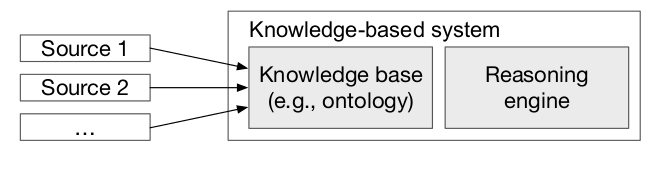
\includegraphics[width = 0.75\linewidth]{KG}
    \caption{Struttura di un KG \cite{KGDefinition}}
    \label{fig:KG}
\end{figure}


\section{Virtual Knowledge Graph}
\label{sec:vkg_description}
I Virtual Knowledge Graph (VKG) applicano al concetto di Knowledge Graph quello di data virtualization. Questo significa che in un VKG l'ontologia non viene materializzata, ma viene dichiarato un insieme di dichiarazioni 
di mapping che permettono di tradurre concetti e proprietà tipiche di un'ontologia in query SQL che vengono eseguite direttamente sulle sorgenti relazionali. Il meccanismo su cui si basa questa riscrittura è descritto 
anche dalla figura \ref{fig:VKGRewriting}.

Un Virtual Knowledge Graph presenta il vantaggio di avere informazioni sempre aggiornate nell'ontologia dato che la query è eseguita direttamente sulle fonti sottostanti, ma, allo stesso tempo, ha performance 
mediamente peggiori rispetto alla sua controparte materializzata, specialmente nei casi in cui i mapping tendano ad essere particolarmente complessi \cite{VKGMedical}

Da un punto di vista più formale possiamo considerare la specifica di un Virtual Knowledge Graph come una tupla $P = (O, M, S)$ dove abbiamo:
\begin{itemize}
    \item Ontologia $O$: rappresentazione a grafo del dominio in analisi con un vocabolario rappresentativo del dominio. Questo grafo è anche arricchito con informazioni riguardanti classi rappresentate nel grafo, le loro pro
        proprietà e la gerarchia tra esse che permette di inferire nuova conoscenza a partire dalle informazioni che già si hanno.
        In questo modo viene implementata una separazione tra i dettagli di basso livello delle fonti e la visione d'insieme data dall'ontologia che permette così anche a persone esperte nel campo, ma non nell'integrazione 
        dei dati, di ricavare informazioni. 
        
        In particolare W3C presenta vari standard per la rappresentazione delle ontologie. Tra questi i principali sono RDFS e OWL, entrambi basati sullo standard RDF (Resource Description Network) usato per descrivere grafi e al 
        fine di interrogare questo grafo lo standard è SPARQL.
    \item Mapping $M$: insieme di affermazioni che specifica come le classi e le proprietà presenti nell'ontologia siano popolate da dati provenienti dalle sorgenti. Formalmente, dato lo schema di un database $S$ e 
        un'ontologia $O$, un'affermazione di mapping tra $S$ e $O$ è un'espressione in una di queste forme:
        \[ \phi(x) \leadsto (f(x) \ \textrm{rdf:type A}) \]
        \[\phi(x, x') \leadsto (f(x) \ P \ f'(x'))\] 
        dove $f$ è un costruttore di termini RDF ovvero una funzione che mappa una tupla di un database a una URI o un letterale RFD.
        In altre parole, tutte le tuple del database vengono tradotte fornendo informazioni o sul tipo di dato o su relazioni di tipo soggetto-predicato-oggetto
        Lo standard per i mapping tra RDF e database relazionali fornito da W3C è R2RML.
    \item Schema $S$: struttura delle sorgenti dati, tipicamente database relazionali. Nel caso di sorgenti eterogenee tra loro è sempre possibile utilizzare uno strumento di federazione come Dremio o Denodo che espone tutte
        le sorgenti come se fossero parte di un unico database relazionale \cite{VKGMedical}.
\end{itemize}

A questo punto possiamo definire un'istanza di un Virtual Knowledge Graph come la coppia $(P, D)$, dove $P = (O, M, S)$ è la specifica di un VKG istanziata su un database $D$ che rispetta lo schema $S$.
Dati $M$ e $D$ le triple generate applicando $M$ su $D$ costituiscono il grafo RDF che esplicita il significato semantico dell'intero sistema.

Se vogliamo caratterizzare un Virtual Knowledge Graph sotto il punto di vista della logica descrittiva allora possiamo considerare l'ontologia come un TBox e le informazioni ricavate dalle sorgenti 
tramite i mapping come l'ABox \cite{OBDA} \cite{VKGOverview}. 


\begin{figure}[ht]
    \centering
    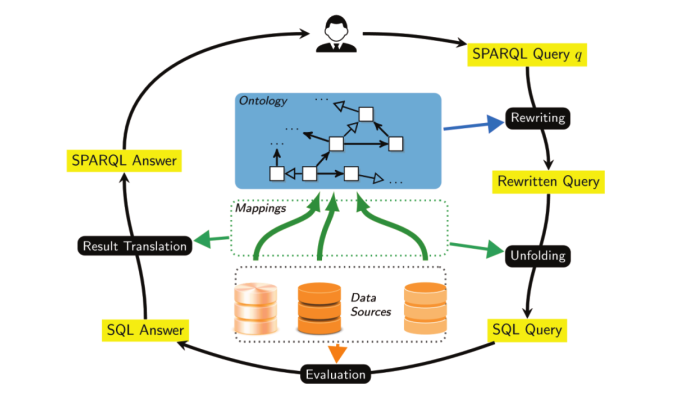
\includegraphics[width = 0.8\linewidth]{VKGRewriting.png}
    \caption{Riscrittura di una query in un VGK \cite{VKGOverview}}
    \label{fig:VKGRewriting}
\end{figure}


\section{Il Virtual Knowledge Graph system Ontop}
\label{sec:vkg_ontop}
Ontop è un Virtual Knowledge Graph system open-source sviluppato dalla Libera Università di Bolzano e supportato commercialmente dall'azienda Ontopic s.r.l. . 
Riceve inoltre contributi importanti dalla Birkbeck, Università di Londra.

\subsection{Architettura del sistema}
Possiamo considerare il sistema Ontop come strutturato su quattro livelli descritti di seguito e riassunti in figura \ref{fig:OntopArchitecture}.
\subsubsection*{Input}
Ontop supporta gli standard W3C in materia di ontologie e Knowledge Graph; in particolare supporta RDF 1.1 come modello per i grafi, RDFS e OWL 2 QL per le
ontologie, la maggior parte dei costrutti presenti in SPARQL 1.1 e R2RML e un sistema di mapping di Ontop, che può essere tradotto in R2RML, per i mapping.

Ontop supporta i maggiori database relazionali tra cui PostgreSQL, MySQL, H2, DB2, Oracle, \dots tramite JDBC e può anche essere utilizzato con federazioni come 
Dremio o Denodo. Inoltre, nonostante sia un VKG system permette di materializzare il grafo RDF se necessario \cite{OntopArchitecture}.

\subsubsection*{Core system}
Parte centrale del sistema che si occupa della traduzione, ottimizzazione ed esecuzione delle query. Alcuni dei dettagli di questo meccanismo sono descritti nella
sezione successiva \ref{sec:ontop_iq}.
\subsubsection*{API}
Ontop può essere utilizzato come libreria Java disponibile tramite Maven ed implementa due API:
\begin{itemize}
    \item OWL API: implementazione di riferimento per la gestione di ontologie OWL.
    \item Sesame: standard de-facto per la gestione di dati in formato RDF. In particolare, Ontop implementa l'interfaccia Sesame SAIL (Storage And Inference Layer) che supporta 
        inferenza e database relazionali.
\end{itemize}
\subsubsection*{Applicazioni}
Ontop supporta anche applicazioni che permettono all'utente finale di eseguire query SPARQL in modo facilitato. Tra queste si citano in particolare: il plugin per Protege basato sull'API OWL,
che fornisce uno strumento grafico per l'editing dei mapping, l'esecuzione di query SPARQL, materializzazione delle triple RDF, \dots e la piattaforma Optique che utilizza Ontop come motore centrale 
aggiungendo un interfaccia user-friendly per la creazione e visualizzazione di query.

\begin{figure}[ht]
    \centering
    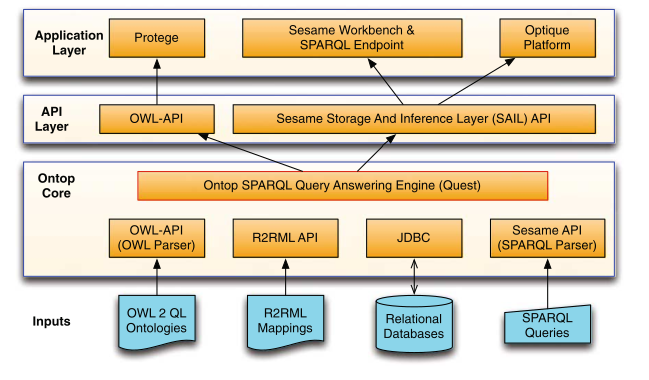
\includegraphics[width=0.75\linewidth]{OntopArchitecture.png}
    \caption{Struttura di Ontop \cite{OntopArchitecture}}
    \label{fig:OntopArchitecture}
\end{figure}

\subsection{Intermediate Query language}
\label{sec:ontop_iq}
Le prime versioni di Ontop erano inizialmente basate su Datalog come motore interno per la traduzione delle query. 
Questa soluzione, sufficiente per la traduzione di query semplici basate sull'unione di query congiuntive, risulta però inadatta per la traduzione di un frammento più grande di SPARQL 
che supporta funzionalità non monotone come OPTIONAL, modificatori di cardinalità come DISTINCT e aggregazione. Per questo con la versione v4, Ontop ha adottato uan struttura dati interna diversa 
chiamata Intermediate Query (IQ) che fornisce una rappresentazione uniforme sia per le query SPARQL eseguite dagli utenti che per le query SQL dei mapping.
Sostanzialmente un IQ è una rappresentazione tramite un albero radicato di un'espressione algebrica dove quest'algebra è un compromesso tra l'algebra di SPARQL da una parte e l'algebra relazionale tipica 
dei database relazionali dall'altra. \cite{Ontop}

Prima di definire più nel dettaglio quest'algebra è necessario spiegare alcuni altri termini ed in particolare:
\begin{itemize}
    \item Termine: per termine indichiamo qualsiasi variabile, costante (incluso NULL) o termine funzionale costruito a partire da variabili o costanti usando simboli funzionali di SPARQL, SQL o interni
    \item Sostituzione: per sostituzione intendiamo un'espressione della forma \linebreak
        $x_1/\mu_1 , \dots , x_n/\mu_n $ dove $x$ corrisponde ad una variabile e $\mu$ ad un termine usato o per la proiezione o per l'aggregazione.
\end{itemize} 
\noindent
I nodi che compongono un albero IQ possono essere di due tipi: \cite{IQ}
\subsubsection*{Nodi foglia} 
Tra i nodi che compongono le foglie dell'albero i più interessanti sono:
    \begin{itemize}
        \item Intensional data node: nodo "prototipo" che ci si aspetta venga sostituito da un IQ; è usato principalmente per rappresentare triple e quadruple in RDF.
        \item Extensional data node: simile a un intensional data node con la differenza che non deve essere necessariamente essere sostituito (ad esempio se rappresenta il nome di una tabella).
        \item Empty node: può essere visto come uno specifico tipo di data node che rappresenta un insieme vuoto di tuple.
        \item Native node: è definito a partire da una query nativa (e.g. una query SQL) ed esplicita i tipi delle variabili ritornate dalla query stessa. Questo tipo di nodo viene generato alla fine 
            della riformulazione e non è usata nei mapping.
    \end{itemize}
\subsubsection*{Nodi interni} 
I nodi interni dell'albero risultano essere più interessanti rispetto alle foglie in quanto rappresentano quelle che sono le operazioni possibili e che devono essere tradotte tra SPARQL e SQL. Tra queste abbiamo:
    \begin{itemize}
        \item Filter node: filtra il proprio nodo figlio in base ad una condizione booleana specificata.
        \item Inner join node: natural join tra gli $n$ figli del nodo sui quali può anche essere applicata una condizione booleana di join. Se questa condizione non è specificata allora il risultato è un cross-join.
        \item Left join node: rappresentazione del left outer join tra i due figli del nodo, eventualmente con condizione di join.
        \item Union node: unione degli $n$ figli opzionalmente preceduta da un'operazione di proiezione.
        \item Construction node: rappresenta la sequenza di tre operazioni: la proiezione, l'applicazione di una funzione al valore di ogni tupla restituita e, infine, la rinomina delle variabili dove
            ognuna di queste tre operazioni è opzionale.
        \item Aggregation node: definito dall'insieme di variabili su cui viene eseguita l'aggregazione e da una sostituzione per definire le nuove variabili ricavate dalle funzioni di aggregazione. Proietta esclusivamente le variabili
            su cui è stata eseguita la proiezione e quelle risultanti dalla rinomina delle funzioni di aggregazione.
        \item Slice node: contiene un limite e/o un offset usati per eliminare un certo numero di tuple dal risultato.
        \item Distinct node: mantiene una singola occorrenza per ogni tupla.
        \item Order by node: ordine le tuple presenti in base ad una lista di comparatori. I valori vengono ordinati in base al primo comparatore e, solo in caso di valori uguali, viene usato il secondo comparatore e così via.
            L'operatore segue una semantica NULL FIRST ASC / NULL LAST DESC. 
    \end{itemize}

\begin{comment}
Formalmente quest'algebra è definita come:
\begin{equation}
    \begin{split}
        \phi := &P(t) \ | \ PROJ_\tau^x \ \phi \ \ | \ AGG_\tau^x \ \phi \ \ | \  DISTINCT \ \phi \ \ | \ ORDERBY_x \ \phi \ \ | \\
                &SLICE_i,j \ \phi \ \ |\ FILTER_\beta \ \phi \ \ | \ JOIN_\beta (\phi_1, \dots, \phi_k ) \ | \\
                &LEFTJOIN_\beta(\phi_1, \phi_2) \ | \ UNION(\phi_1, \dots, \phi_k ) 
    \end{split}
\end{equation}
dove $P$ è il nome di una relazione, $t$ è una tupla di termini, $x$ è una tupla di variabili, $\tau$ è una sostituzione, $i,j$ sono numeri naturali che descrivono il limite e l'offset e $\beta$ è un termine booleano.

Nonostante la maggior parte del processamento della query sia poi lasciato al DBMS (Ontop modella ogni dialetto individualmente usando Java factory specifiche per ogni dialetto), IQ si occupa di tradurre aspetti della query SPARQL nel loro equivalente SQL. Questo è scontato per alcuni costrutti dove sia sintassi che 
semantica sono consistenti, mentre per altri i due linguaggi hanno comportamenti diversi. Di seguito si elencano alcune delle differenze principali tra i due linguaggi: \cite{Ontop}
\begin{itemize}
    \item tipizzazione: SQL è staticamente tipizzato ovvero tutti i valori in una colonna devono essere dello stesso tipo mentre SPARQL usa tipi dinamici. Questo significa che in SPARQL una funzione può accettare tipi diversi mentre questi
        sono fissi in SQL (ad esempio numeric\_add)
    \item ordinamento: SPARQL deve definire un ordine predefinito per IRI, blank nodes, variabili e letterali mentre in SQL è solamente necessario scegliere il modificatore e specificare l'ordine per NULL
    \item condizione di join: al fine di effettuare un join in SPARQL i due mapping devono essere compatibili ovvero devono condividere la stessa variabile o lo stesso termini RDF (e quindi hanno la stesso tipo e valore lessicale). Per quanto 
        riguarda SQL invece non è necessario che gli argomenti siano dello stesso tipo e possono anche avere valori lessicali diversi (ad esempio timestamps con diversi fusi orari)
    \item dialetti: mentre SPARQL ha sintassi e semantica standard, SQL è vendor-specific 
\end{itemize}
\end{comment}
Durante la traduzione l'albero IQ subisce pesanti operazioni di ottimizzazione basate su tecniche derivate dalla Semantic Query Optimization che sono fondamentali per una riscrittura efficiente. Una loro descrizione più approfondita esula però degli obiettivi di questo elaborato.
Oltre alle ottimizzazioni, il sistema è reso più performante dal delegare al DBMS specifico una buona parte della computazione della query. In particolare Ontop modella ogni dialetto SQL individualmente usando Java factory specifiche per ogni ognuno di essei ovvero 
modella i tipi, le convenzioni nei nomi di attributi e tabelle, la semantica delle funzioni, la struttura dei data catalog, \dots. 

\subsection{Esempi di utilizzo}
Data la distribuzione di Ontop come progetto open-source con licenza Apache2 è impossibile conoscerne tutti i casi di utilizzo. Nonostante ciò esistono comunque casi documentati di uso di questo VGK system sia in ambito commerciale che pubblico. Di seguito ne descriviamo due di particolare interesse. \cite{Ontop}
\subsubsection*{Open Data Hub-Virtual-Knowledge-Graph}
Open Data Hub-Virtual Knowledge Graph nasce come un progetto congiunto tra il NOI Techpark e Ontopic al fine di pubblicare e rendere disponibili i dati del'Alto Adige su turismo e mobilità. Inizialmente questi dati erano accessibili attraverso un'API JSON, ma l'introduzione di un VKG, con annesso endopoint SPARQL, ha
reso questo sistema estremamente più potente e flessibile.
\subsubsection*{UNiCS}
UNiCS è una piattaforma sviluppata da SIRIS Academic che integra dati provenienti da fonti come la commissione europea, governi nazionali e regionali e specifiche università al fine di aiutare università ed istituti di ricerca nel prendere scelte informate e supportate da dati. Tutti questi dati sono disponibili 
tramite un'ontologia che può essere interrogata tramite un endpoint SPARQL e i cui risultati possono poi essere visualizzati tramite grafiche e statistiche di più facile interpretazione \cite{UniCS}.

